\chapter{Regularization}
Le tecniche di regolarizzazione puntano a ridurre l'errore della loss function sul validation set e sul test set al costo di un
incremento ragionevole sul train error.

La regolarizzazione comprende qualsiasi tecnica che effettua una modifica nel processo di apprendimento al fine di
ridurre l'errore di generalizzazione, ma non il train error.

La regolarizzazione può avvenire:
\begin{itemize}
  \item Direttamente: aggiungendo vincoli ai parametri o alla funzione obiettivo
  \item Indirettamente: aggiungendo dati e introducendo rumore nei dati
\end{itemize}

Un regolarizzatore efficace riduce significativamente la varianza mentre non aumenta molto il bias.

\section{Norm Penalities}
Si limita la capacità del modello aggiungendo una penalità $\Omega(\theta)$ alla funzione obiettivo $J$.
%
\begin{align*}
  \tilde{J}(\theta) = J(\theta) + \alpha \Omega(\theta)
\end{align*}
%
$\alpha \in [0, \inf)$ è un iperparametro che pesa il contributo della \textbf{norm penalty} nella funzione obiettivo.

Solitamente la penalty $\Omega$ penalizza solo i pesi della trasformazione affine di ogni layer.
I bias nella trasformazione affine richiedono meno dati per fittare, quindi non vengono regolarizzati.

Più parametri ci sono nel modello più questi sono sensibili a varianza, e quindi creano più instabilità nel modello.

- somma assoluta dei pesi
\begin{align*}
  \Omega(w, b) = \sum_{w_j}|w_j|
\end{align*}

- somma quadratica dei pesi
\begin{align*}
  \Omega(w, b) = \sqrt{\sum_{w_j}|w_j|^2}
\end{align*}

Data la funzione obiettivo seguente
\begin{align*}
  \tilde{J}(w; X, y) = \frac{\alpha}{2} w^T w + J(w; X, y)
\end{align*}

Il gradiente é:
\begin{align*}
  \nabla_w \tilde{J}(w; X, y) = \alpha w + \nabla_w J(w; X, y)
\end{align*}

La regola di aggiornamento dei pesi usando la norma L2 diventa la seguente
\begin{align*}
  w & = w - \varepsilon \big( \alpha w + \nabla_w J(w; X, y) \big)   \\
    & = (1 - \varepsilon \alpha) w + \varepsilon \nabla_w J(w; X, y)
\end{align*}

\section{Data Augmentation}
Il miglior modo per ottenere una migliore generalizzazione è usare più dati per l'addestramento.
Spesso i dati sono limitati e necessitano di essere etichettati.

Una soluzione è quella di generare nuovi dati artificialmente riutilizzando quelli già presenti applicando delle trasformazioni o aggiungendo rumore.

\begin{itemize}
  \item Flip (Horizontal, Vertical)
  \item Random Noise Injection (all'input o ai pesi)
  \item Rotations
  \item Cropping
  \item Color Modification
\end{itemize}

E' utile effettuare l'addestramento sia sul dataset esteso che sul dataset di partenza per poterne valutare i vantaggi.

\section{Label Smoothing}
Può capitare che alcuni dataset presentino errori nelle etichette. Questi possono essere dovuti a errori umani o al risultato di
algoritmi di labelling automatico. Per gestire questi possibili errori si modella esplicitamente il rumore nelle label.

Il label smoothing è una tecnica che si basa su una softmax con k valori di output in cui 0 e 1 vengono sostituiti nel seguente modo:
\begin{align*}
  0 \Rightarrow \frac{\varepsilon}{k - 1} \qquad 1 \Rightarrow 1 - \varepsilon
\end{align*}
in cui $\varepsilon$ è la probabilità che la label sia corretta.

\section{Early Stopping}
L'early stopping è una tecnica di regolarizzazione che evita di addestrare eccessivamente il modello sul train set in modo da evitare l'overfitting.

Ad ogni epoca viene osservato il validation error e vengono salvati i parametri del modello migliore.
Dopo un numero di iterazioni (patience) che il validation error continua a peggiorare l'algoritmo si ferma.

Esistono più strategie per sfruttare questa tecnica:
\begin{enumerate}
  \item {
        \begin{itemize}
          \item Si esegue l'early stopping
          \item Viene riaddestrato il modello fino al punto in cui si è fermato con i parametri ottenuti
        \end{itemize}
        }
  \item {
        \begin{itemize}
          \item Si esegue l'early stopping
          \item Si continua l'addestramento con i parametri ottenuti utilizzando solo il validation set
        \end{itemize}
        }
\end{enumerate}

\section{Parameter Tying and Sharing}


\section{Multitask Learning}
Il multitask learning è un approccio in cui si cerca di imparare diversi tasks contemporaneamente.
Permette di migliorare la generalizzazione mettendo in comune degli esempi per più task.

Il task aggiuntivo aggiunge dei vincoli ai parametri dei layer condivisi e permette di imparare una rappresentazione condivisa e quindi di ottenere una maggiore generalizzazione.

L'architettura di una rete multitask è comunemente composta da due parti:
i \textbf{task-specific layers} che traggono beneficio solo dagli esempi definiti per i task specifici e
gli \textbf{shared layers} che traggono beneficio dai dati messi in comune.

\begin{figure}[ht]
  \centering
  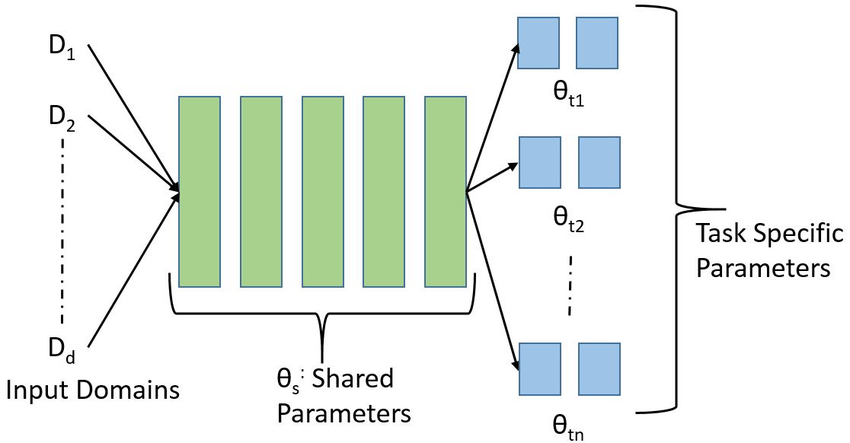
\includegraphics[width=0.8\linewidth]{images/multitask.png}
  \label{img:multitask}
  \caption{Schema di rete multitask \cite{img:multitask}}
\end{figure}

E' necessario trovare il giusto insieme di parametri da condividere: una scarsa condivisione di parametri non risulta efficace, mentre un'eccessiva condivisione potrebbe portare a ottenere 
prestazione peggiori \cite{crawshaw2020multi}. 

Il miglioramento della generalizzazione avviene solo se i task hanno qualcosa in comune (correlazione).


\section{Bagging}
Il bagging (bootstrap aggregation) una tecnica di \textbf{ensemble method} che riduce 
l'errore di generalizzazione combinando diversi modelli.

\begin{figure}[ht]
  \centering
  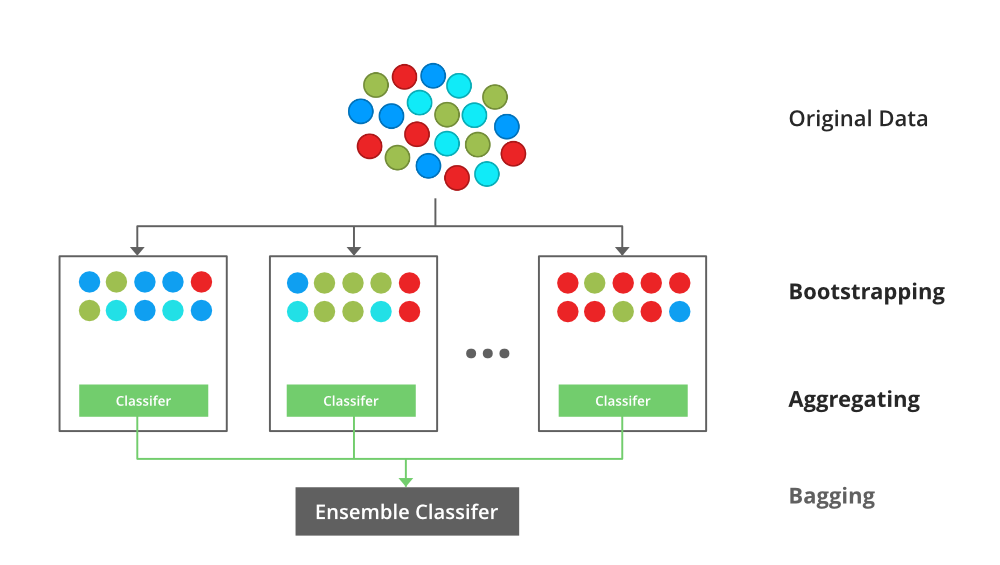
\includegraphics[width=0.9\linewidth]{images/bagging.png}
  \label{img:bagging}
  \caption{Schema di funzionamento del bagging \cite{img:bagging}}
\end{figure}

Viene effettuato l'addestramento di k modelli diversi su k insiemi del training set ottenuti tramite un campionamento casuale con sostituzione\footnotemark (bootstrap).
I risultati vengono aggregati (aggregation) calcolando una media (soft voting) nel caso di regressione o tramite una votazione (hard voting) nel caso di classificazione.

Se un singolo membro dell'ensemble fa degli errori, l'ensemble funzionerà meglio dei membri.

Solitamente il numero di modelli è piccolo poiché risulta oneroso gestirne tanti in termini di computazione e di memoria. 
E' meglio avere un numero di modelli dispari per non avere casi di parità.

\footnotetext{Nel campionamento casuale con sostituzione i campioni possono essere scelti più volte}

\section{Dropout}
